
\section {Introduction}

One of the primary high-level strategic inputs to developing the {\it System AI\&T and Commissioning Plan} (\citeds{LSE-79}) are the construction completeness requirements for the Construction Completeness Review (CCRs).  In (\citeds{LSE-79}), the Project has identified 10 general requirements for "construction completeness", including one requirement for "operations readiness", these are summarized as:

\begin{itemize}
        \item Verification of LSST System Requirements (\citeds {LSE-29}) and survey performance as described in SRD (\citeds {LPM-17})
        \item Verification of the Observatory System Specifications (\citeds {LSE-30})
        \item Verification of Data Processing, Products and User Services
        \item Demonstrating Science Data Quality Assessment (SDQA)
        \item Conduct a Science Validation Survey
        \item Demonstrate the system state is recorded and archived for each observation
        \item Verify Education and Public Outreach has met its requirements and construction scope
        \item Operational procedures and documented and accessible
        \item Provided a record of the as-built system, including modification since the as-build and non-compliance
        \item Demonstrate Rubin Operations Team readiness.
\end{itemize}

At the conclusion of the Rubin Observatory Construction Project's commissioning phase, a series of CCRs will be undertaken by an external panel jointly appointed by the DOE and NSF in consultation with the Project Team. The successful completion of the CCRs will signify the end of the NSF MREFC-funded construction project and DOE Commissioning. The CCRs are consistent with the NSF guidance given in the {\it Major facilities Guide} (\citeds{NSF-19-68}) Sections $2.4.2.1$ -- {\it Project Close--out Process}, $3.4.2.15$ -- {\it Commissioning}, $4.4$ -- {\it System Integration, Testing and Acceptance} and $4.5$ -- {\it Documentation Requirements}.

The series of CCRs will consist of four meetings, as shown in Figure XXX.
\begin{figure}[htbp]
\begin{center}
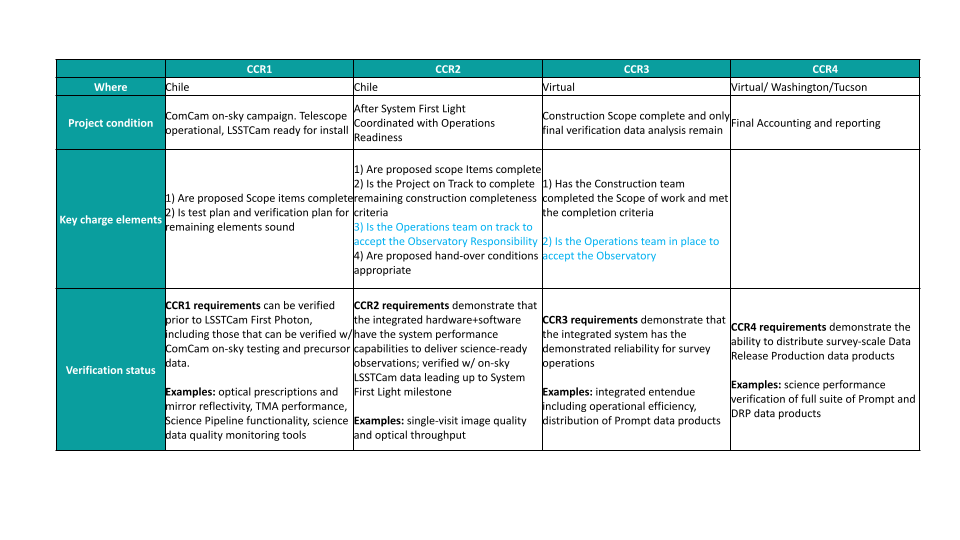
\includegraphics[width=1\textwidth]{./CCRs_overview.png}
\caption{Construction Completeness Review overview}
\label{CCRs_overview}
\end{center}
\end{figure}


The CCRs will cover two aspects: 
 1) The evaluation of the Rubin Construction Project completeness criteria and 
 2) the Rubin Observatory Operations team's readiness to receive the construction deliverables and begin planned operations for conducting the Legacy Survey of Space and Time -- the 10-year science survey for which the Rubin Observatory was designed and constructed to perform.

In this document, we collect together and detail the elements that constitute the criteria for construction completeness and operations readiness. 
Each topic has its own or will reference well-defined requirements -- in some cases, these include goals and stretch goals -- each will have the relevant supporting documentation for performance against the requirement. For those requirements that specify performance after some period of operations, the basis of the estimated projected performance will be provided. Unless otherwise specified, functional requirements will be verified by direct test, and performance requirements will be verified by direct test, analysis, or some combination thereof.  For each requirement, there will either be a clean pass or a waiver process that documents why it is acceptable to proceed to operations (or the reason we must postpone the transition to operations).

Some topics summarized in this document are already covered by existing verification plans.  Some functional requirements (and any accompanying goals and stretch goals) are still in review (at the time of this document version) -- in those cases, the requirements and associated verifications are being developed together to ensure clarity and crisp requirements for verifiability. Some topics, such as the Science Validation surveys, have requirements that are a combination of performance and functionality that do not easily flow directly from the high-level system requirements; in those cases, we identify the minimum requirements and performance that must be met to proceed to operations, along with a range of goals and stretch goals and the accompanying rationale.

For each of the general CRR requirements, we provide:

\begin{itemize}
	\item The statement of the requirements;
	\item An expansion of objective and intent;
	\item Specific criteria for completeness;
	\item Indication of any pre--Operation interactions; and
	\item The expected delivered artifacts.
\end{itemize}
	